\documentclass{standalone}
\usepackage{tikz}
\usetikzlibrary{intersections}
\begin{document}

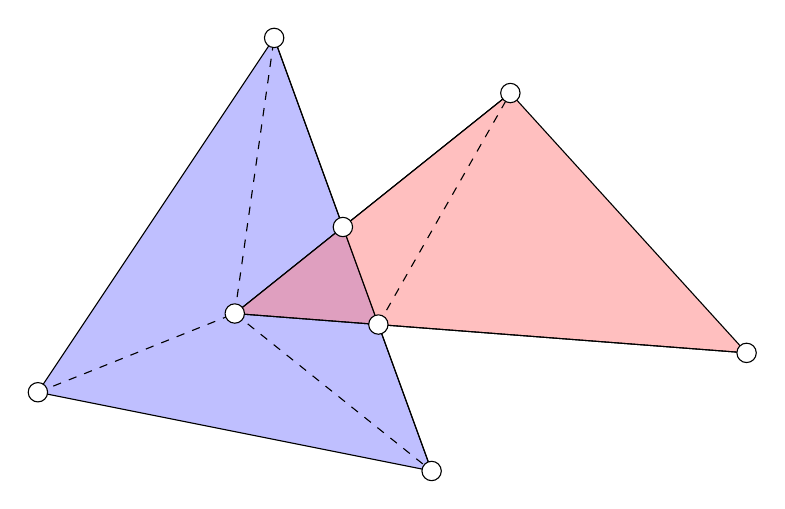
\begin{tikzpicture}[every node/.style={circle,draw=black, fill=white, inner sep=0pt,minimum size=7pt}]
  % Simplex 1
  \coordinate (A) at (0,0);
  \coordinate (B) at (3,4.5);
  \coordinate (C) at (5,-1);

  % Simplex 2
  \coordinate (D) at (2.5,1);
  \coordinate (E) at (6,3.8);
  \coordinate (F) at (9,.5);

  \draw[fill=blue!50!white, fill opacity=.5] (A) -- (B) -- (C) -- (A);
  \draw[fill=red!50!white, fill opacity=.5] (D) -- (E) -- (F) -- (D);

  \draw[name path=B--C] (B) -- (C);
  \draw[name path=D--E] (D) -- (E);
  \draw[name path=D--F] (D) -- (F);

  \path[name intersections={of=B--C and D--E, by=G}];
  \path[name intersections={of=B--C and D--F, by=H}];

  \draw[dashed] (A) -- (D);
  \draw[dashed] (D) -- (B);
  \draw[dashed] (D) -- (C);
  \draw[dashed] (H) -- (E);

  \node (g) at (G) {};
  \node (h) at (H) {};

  % nodes for simplex (1)
  \node (a) at (A) {};
  \node (b) at (B) {};
  \node (c) at (C) {};

  % nodes for simplex (2)
  \node (d) at (D) {};
  \node (e) at (E) {};
  \node (f) at (F) {};
\end{tikzpicture}
\end{document}
